\documentclass[
]{jss}

\usepackage[utf8]{inputenc}

\providecommand{\tightlist}{%
  \setlength{\itemsep}{0pt}\setlength{\parskip}{0pt}}

\author{
H. Sherry Zhang\\Monash University \And Dianne Cook\\Monash University
\AND Ursula Laa\\University of Natural Resources and Life Sciences
\AND Nicolas Langrené\\CSIRO Data61 \AND Patricia
Menéndez\\Monash University \AND
}
\title{\pkg{cubble}: An R Package for Structuring Spatio-temporal Data}

\Plainauthor{H. Sherry Zhang, Dianne Cook, Ursula Laa, Nicolas
Langrené, Patricia Menéndez}
\Plaintitle{cubble: An R Package for Structuring Spatio-temporal Data}

\Abstract{
The abstract of the article.
}

\Keywords{spatio-temporal data, \proglang{R}}
\Plainkeywords{spatio-temporal data, R}

%% publication information
%% \Volume{50}
%% \Issue{9}
%% \Month{June}
%% \Year{2012}
%% \Submitdate{}
%% \Acceptdate{2012-06-04}

\Address{
          }

% Pandoc citation processing

% Pandoc header

\usepackage{amsmath} \usepackage{array}

\begin{document}

\newpage

\hypertarget{introduction}{%
\section{Introduction}\label{introduction}}

\textbf{Motivation}

Many data structures have been proposed for spatial (\pkg{sf} by
\citet{sf}) and temporal (\pkg{tsibble} by \citet{tsibble}) data in the
R community, while less has been done for spatio-temporal data. The lack
of such tools could potentially because analysts usually treat the
spatial and temporal dimension of the data separately, without realising
the need to create a new data structure. While this approach follows the
third tidy data principal \citep{tidydata} (\emph{Each type of
observational unit forms a table}), analysts always need to manually
join results from different observational units or combining multiple
tables into one for downstream analysis. This additional step doesn't
add new operations into the data but can be error prone. \newline

\textbf{Existing packages}

Currently, available spatio-temporal data structure in R includes:
\pkg{spacetime} \citep{spacetime}, which proposes four space-time
layouts: Full grid (STF), sparse grid(STS), irregular (STI), and
trajectory (STT). The data structure it uses is based on \pkg{sp}
\citep{sp} and \pkg{xts} \citep{xts}, both of which has been replaced by
more recent implementations. \pkg{spatstat} \citep{spatstat} implements
a \texttt{ppp} class for point pattern data; and more recent,
\pkg{stars} \citep{stars} implements a spatio-temporal array with the
dplyr's data cube structure \pkg{cubelyr} \citep{cubelyr} as its
backend. While these implementations either store spatial and temporal
variables all in a single table, hence duplicate the spatial variables
for each temporal unit; or split them into two separate tables that has
the problem of manually joining, mentioned in the previously. None of
these packages enjoy both the benefits of being able to separate
manipulation in the two dimensions while also keep the data object as a
whole. This create a gap in the software development. The requirement
for such a tool is important given the ubiquity of spatio-temporal
vector data in the wild: the Ireland wind data from \pkg{gstat} is an
classic example data that splits variables into spatial
(\texttt{wind.loc}) and temporal (\texttt{wind}) dimension; Bureau of
Meteorology (BoM) provides climate observations that are widely applied
in agriculture and ecology study; air pollution data. \newline

\textbf{Our new data structure for spatio-temporal data} This paper
describes the implementation of a new spatio-temporal data structure:
\pkg{cubble}. \pkg{cubble} implements a relational data structure that
uses two forms to manage the switch between spatial and temporal
dimension. With this structure, users can manipulate the spatial or
temporal dimension separately, while leaves the linking of two
dimensions to \textbackslash pkg\{cubble\textbackslash pkg\{. The
software is available from the Comprehensive R Archive Network (CRAN) at
{[}CRAN link{]}. \newline

\textbf{Section division}

The rest of the paper will be divided as follows: {[}complete when the
paper structure is more solid{]}

\newpage

\hypertarget{the-cubble-package}{%
\section{The cubble package}\label{the-cubble-package}}

Spatio-temporal data usually come in various forms and Figure
\ref{fig:cubble-diagram} shows four examples of this. No matter which
form the data is in, these formats share some common components that
characterise spatio-temporal data. A spatial identifier (\texttt{id} in
the diagram) is the unique identifier of each site. The temporal
identifier (\texttt{t} in the diagram) prescribes the time stamp each
site is recorded. Coordinates, comprising of latitude and longitude
(\texttt{lon} and \texttt{lat} in the diagram), locates each site on the
map. These identifiers will be the building blocks for the data
structure introduced below. Other variables in the data can be
categorised into two groups: spatial variables that are invariant at
each time stamp for every site, i.e.~the name or code of the weather
station and temporal variables that varies with time.

\begin{CodeChunk}
\begin{figure}

{\centering 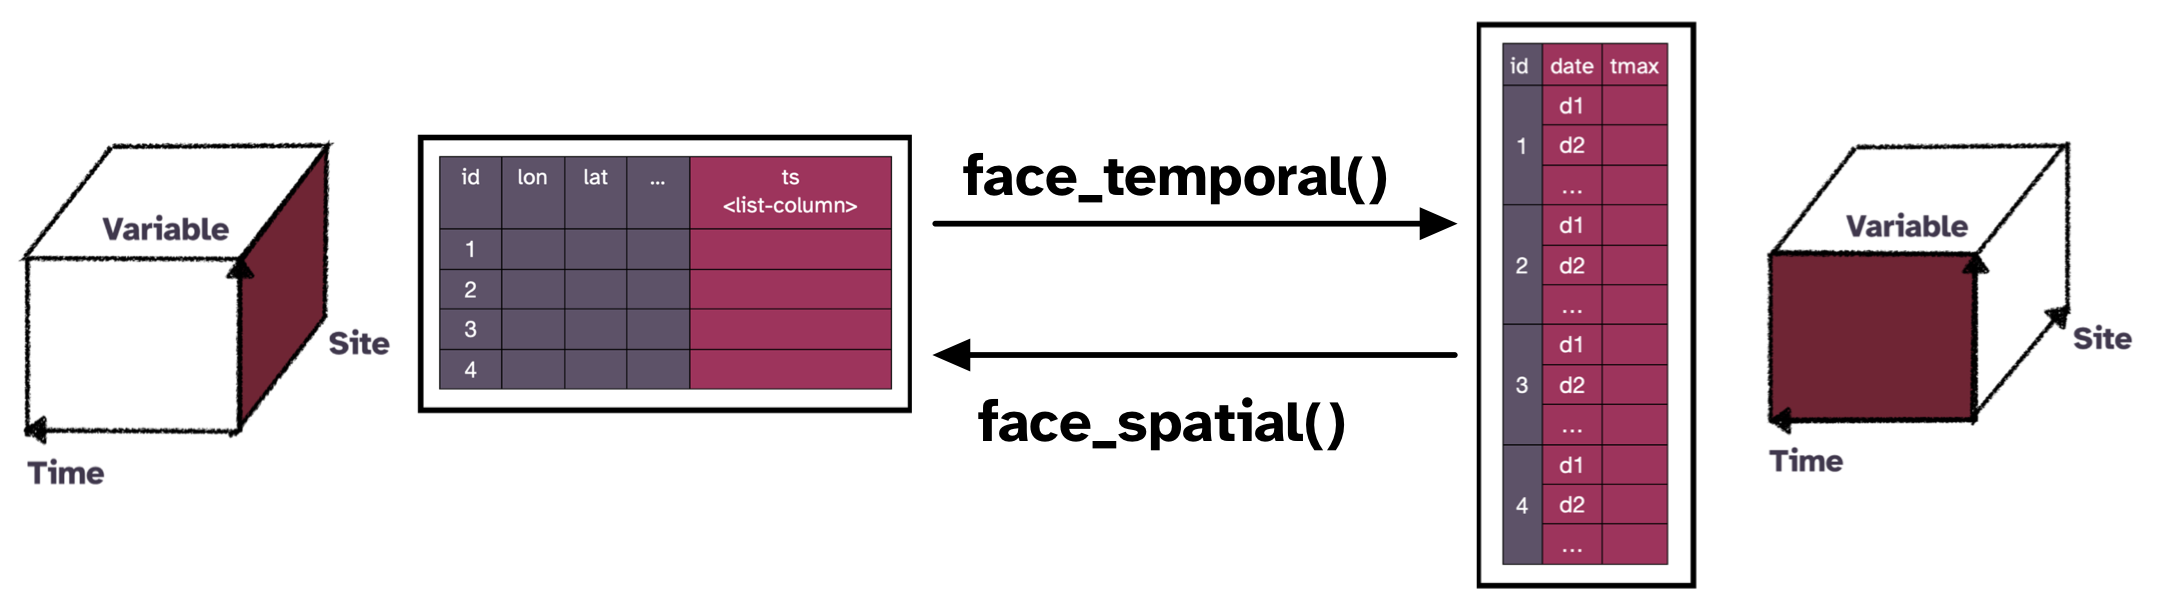
\includegraphics[width=1\linewidth,height=0.15\textheight]{/Users/sherryzhang/Documents/research/paper-cubble/figures/diagram-keynotes/diagram-keynotes.001} 

}

\caption[Illustration of incoming data formats for spatio-temporal data]{Illustration of incoming data formats for spatio-temporal data. (1) Data comes in as a single table; (2) Separate tables for spatial and temporal variables; (3) A single table with all the parameters used to query the database and a separate table for queried data; and (4) Cubical data in array or NetCDF format.}\label{fig:cubble-diagram}
\end{figure}
\end{CodeChunk}

In a cubble, there are two forms: nested form and long form, and Figure
\ref{fig:def-cubble} sketches the two forms along with the associated
attributes. The decision on which form to use is output-oriented,
meaning analysts need to first think about whether the output of a
particular operation is identified only by the spatial identifier, or a
combination of spatial and temporal identifier. The nested cubble is
suitable for working with operations that are only identified by site
and this type of operation can be a pure manipulation of spatial
variables, or a summary of temporal variables by site (i.e.~the output
of counting the number of raining day is only identified by sites and
hence should be performed with the nested form). Underneath the nested
form, a cubble is built from a row-wise dataframe (\texttt{rowwise\_df})
where each site forms a separate group. This structure simplifies the
calculation that involves temporal variables by avoiding the use of
\texttt{map} syntax when working with list-column.

For those operations whose output involves both a spatial and temporal
dimension, long form should be used. The long form is identified by both
the spatial and temporal identifier and adopts a grouped dataframe
(\texttt{grouped\_df}) to forms each site as a group. Spatial variables
are stored separately in a \pkg{tibble} as an special attribute of the
long cubble. This design avoids repeating the spatial variables at each
time stamp while not dropping information from spatial variables.

\begin{CodeChunk}
\begin{figure}

{\centering 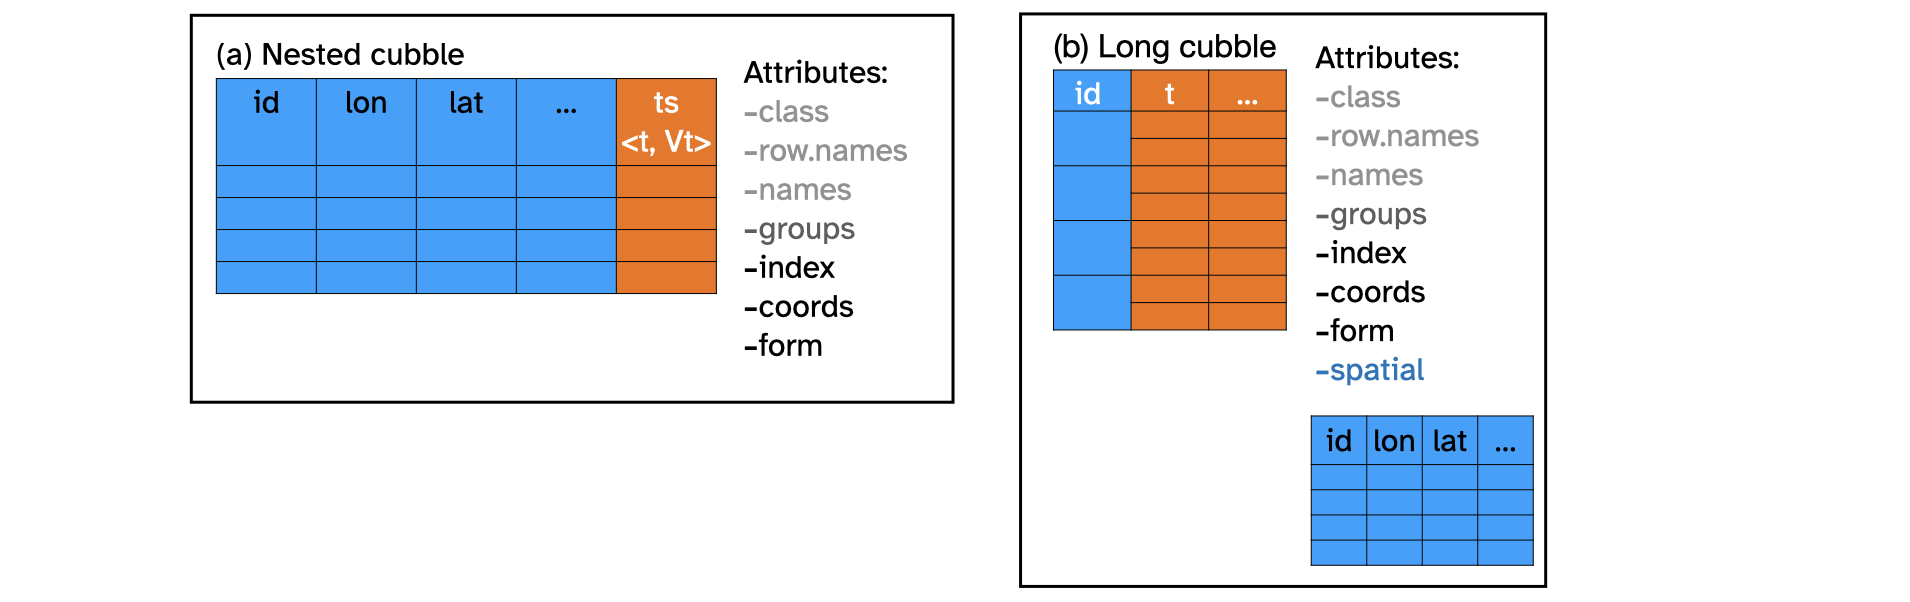
\includegraphics[width=1\linewidth]{/Users/sherryzhang/Documents/research/paper-cubble/figures/diagram-keynotes/diagram-keynotes.002} 

}

\caption[Illustration of nested and long cubble]{Illustration of nested and long cubble.}\label{fig:def-cubble}
\end{figure}
\end{CodeChunk}

\hypertarget{create-a-cubble-in-the-nested-form}{%
\subsection{Create a cubble in the nested
form}\label{create-a-cubble-in-the-nested-form}}

To use functionalities from cubble, data analysts first need to create a
cubble. \texttt{as\_cubble} create a \pkg{cubble} by supplying the three
key components: \texttt{key} as the spatial identifier; \texttt{index}
as the temporal identifier; and a vector of \texttt{coords} in the order
of longitude first and then latitude. The naming of \texttt{key} and
\texttt{index} follows the convention in the \pkg{tsibble} package. The
cubble created by default is in the nested form. Below is an example of
creating a cubble: \newline

\begin{CodeChunk}
\begin{CodeOutput}
# cubble:   id [5]: nested form
# bbox:     [115.97, -32.94, 133.55, -12.42]- check gap on long and lat
# temporal: date [date], prcp [dbl], tmax [dbl], tmin [dbl]
  id            lat  long  elev name           wmo_id ts                
  <chr>       <dbl> <dbl> <dbl> <chr>           <dbl> <list>            
1 ASN00009021 -31.9  116.  15.4 perth airport   94610 <tibble [366 x 4]>
2 ASN00010311 -31.9  117. 179   york            94623 <tibble [366 x 4]>
3 ASN00010614 -32.9  117. 338   narrogin        94627 <tibble [366 x 4]>
4 ASN00014015 -12.4  131.  30.4 darwin airport  94120 <tibble [366 x 4]>
5 ASN00015131 -17.6  134. 220   elliott         94236 <tibble [366 x 4]>
\end{CodeOutput}
\end{CodeChunk}

There are a few information in the \pkg{cubble} header: the name of the
\texttt{key} variable, bbox, and also the name of variable nested in the
\texttt{ts} column. In this example, each site is identifier is
\texttt{id} and the number in the bracket means there are 5 unique
\texttt{id} in this dataset. The bbox in the second row gives the range
of the coordinates. The temporal variables are all nested in the
\texttt{ts} column, but it could be useful to know the name these
variables. The third row in the cubble header shows these names and in
this example this includes: precipitation, \texttt{prcp}, maximum
temperature, \texttt{tmax}, and minimum temperature, \texttt{tmin}.

\hypertarget{stretch-a-nested-cubble-into-the-long-form}{%
\subsection{Stretch a nested cubble into the long
form}\label{stretch-a-nested-cubble-into-the-long-form}}

The long cubble is suitable to manipulate the time dimension of the
data. The function \texttt{stretch()} switches the nested cubble into
the long cubble by first extracts all the spatial variables into a
separate tibble and store in the \texttt{spatial} attribute and then
unnests the \texttt{ts} column:

\begin{CodeChunk}
\begin{CodeOutput}
# cubble:  date, id [5]: long form
# bbox:    [115.97, -32.94, 133.55, -12.42]- check gap on long and lat
# spatial: lat [dbl], long [dbl], elev [dbl], name [chr], wmo_id [dbl]
   id          date        prcp  tmax  tmin
   <chr>       <date>     <dbl> <dbl> <dbl>
 1 ASN00009021 2020-01-01     0  31.9  15.3
 2 ASN00009021 2020-01-02     0  24.9  16.4
 3 ASN00009021 2020-01-03     6  23.2  13  
 4 ASN00009021 2020-01-04     0  28.4  12.4
 5 ASN00009021 2020-01-05     0  35.3  11.6
 6 ASN00009021 2020-01-06     0  34.8  13.1
 7 ASN00009021 2020-01-07     0  32.8  15.1
 8 ASN00009021 2020-01-08     0  30.4  17.4
 9 ASN00009021 2020-01-09     0  28.7  17.3
10 ASN00009021 2020-01-10     0  32.6  15.8
# ... with 1,820 more rows
\end{CodeOutput}
\end{CodeChunk}

Notice here that the third line in the header now shows the name of
spatial variables rather than the temporal variables.

\hypertarget{tamp-a-long-cubble-back-to-the-nested-form}{%
\subsection{Tamp a long cubble back to the nested
form}\label{tamp-a-long-cubble-back-to-the-nested-form}}

Manipulation on the spatial and temporal dimension can be an iterative
process. Many times, analysts will need to go back and forth between the
nested and long cubble. The \texttt{stretch()} function introduced in
the previous section switches a nested cubble into a long cubble and
function \texttt{tamp()} is its inverse function to switch a long cubble
back to the nested cubble:

\begin{CodeChunk}
\begin{CodeOutput}
# cubble:   id [5]: nested form
# bbox:     [115.97, -32.94, 133.55, -12.42]- check gap on long and lat
# temporal: date [date], prcp [dbl], tmax [dbl], tmin [dbl]
  id            lat  long  elev name           wmo_id ts                
  <chr>       <dbl> <dbl> <dbl> <chr>           <dbl> <list>            
1 ASN00009021 -31.9  116.  15.4 perth airport   94610 <tibble [366 x 4]>
2 ASN00010311 -31.9  117. 179   york            94623 <tibble [366 x 4]>
3 ASN00010614 -32.9  117. 338   narrogin        94627 <tibble [366 x 4]>
4 ASN00014015 -12.4  131.  30.4 darwin airport  94120 <tibble [366 x 4]>
5 ASN00015131 -17.6  134. 220   elliott         94236 <tibble [366 x 4]>
\end{CodeOutput}
\end{CodeChunk}

\hypertarget{migrate-spatial-variables-to-a-long-cubble}{%
\subsection{Migrate spatial variables to a long
cubble}\label{migrate-spatial-variables-to-a-long-cubble}}

As a final data output for modelling or visualisation, spatio-temporal
data is usually expected to be in a single table. Function
\texttt{migrate()} moves the spatial variables from the \texttt{spatial}
attribute into the long cubble:

\begin{CodeChunk}
\begin{CodeOutput}
# cubble:  date, id [5]: long form
# bbox:    [115.97, -32.94, 133.55, -12.42]- check gap on long and lat
# spatial: lat [dbl], long [dbl], elev [dbl], name [chr], wmo_id [dbl]
   id          date        prcp  tmax  tmin  long   lat
   <chr>       <date>     <dbl> <dbl> <dbl> <dbl> <dbl>
 1 ASN00009021 2020-01-01     0  31.9  15.3  116. -31.9
 2 ASN00009021 2020-01-02     0  24.9  16.4  116. -31.9
 3 ASN00009021 2020-01-03     6  23.2  13    116. -31.9
 4 ASN00009021 2020-01-04     0  28.4  12.4  116. -31.9
 5 ASN00009021 2020-01-05     0  35.3  11.6  116. -31.9
 6 ASN00009021 2020-01-06     0  34.8  13.1  116. -31.9
 7 ASN00009021 2020-01-07     0  32.8  15.1  116. -31.9
 8 ASN00009021 2020-01-08     0  30.4  17.4  116. -31.9
 9 ASN00009021 2020-01-09     0  28.7  17.3  116. -31.9
10 ASN00009021 2020-01-10     0  32.6  15.8  116. -31.9
# ... with 1,820 more rows
\end{CodeOutput}
\end{CodeChunk}

In this workflow described above, data objects come into cubble in the
nested form, then various operations on the spatial and temporal
dimension can go back and forth between the nested and long form, and
finally, the data will come out of cubble in the long form for further
modelling or visualisation.

Building from an underlying \texttt{tbl\_df} structure, it is natural to
implement methods available in \texttt{dplyr} to \texttt{cubble}.
Supported methods in the \texttt{cubble} with \texttt{dplyr} generics
includes:

\begin{center}
\begin{tabular}{ | m{5em} | m{15cm}| } 
basics & \textbf{mutate}, \textbf{filter}, \textbf{summarise}, \textbf{select}, \textbf{arrange}, \textbf{rename}, \textbf{left\_join} \\
grouping &  \textbf{group\_by}, \textbf{ungroup}\\
slice family & \textbf{slice\_head}, \textbf{slice\_tail}, \textbf{slice\_sample}, \textbf{slice\_min} and \textbf{slice\_max} \\
\end{tabular}
\end{center}

\pkg{cubble} is also compatible with \pkg{tsibble} in the sense that the
original list-column can be a \texttt{tbl\_ts} object. Duplicates and
gaps should be first checked before structuring the data into a cubble.
If the input data is a \pkg{tsibble} object, the long form cubble is
also a \pkg{tsibble} where users can directly apply time series
operations.

\hypertarget{advanced-features-considerations}{%
\section{Advanced features/
considerations}\label{advanced-features-considerations}}

\hypertarget{hierarchical-structure}{%
\subsection{Hierarchical structure}\label{hierarchical-structure}}

Imposing a clustering structure can be thought of as building a
hierarchical structure where stations are nested within clusters. This
can be useful when there's intrinsic nesting structure in the data
(i.e.~country nested in the continent, county nested in the state) or
there's some clustering. When we have access to both level,
\texttt{switch\_key()} is the function to re-structure the data as one
cluster per row. Temporal observations from different stations while
within the same cluster are bound in the nested column \texttt{ts}.

One thing we hope to do with the cluster is to find the coordinates of
the centroid. These are variables variant to the station but invariant
to the cluster and it would be nice to have a function that structure
each cluster as a row. \texttt{switch\_key()} is the function that does
this: it lets you to specify a new key, say \texttt{cluster} and nests
all spatial variables variant to \texttt{cluster} into a column. Spatial
variables are all nested inside a new column \texttt{.val}. Temporal
observations from different stations while within the same cluster are
bound in the nested column \texttt{ts}.

This structure makes it easy to compute cluster level variable, for
example, the convex hull and the centroid coordinate of each cluster.
These can be amended into the nested form with function
\texttt{get\_centroid}.

After we have got \texttt{cluster\_nested}, spatial and temporal data at
both levels can be easily obtained. Figure \ref{fig:hierachical}
illustrate the relationship between the long and nested form cubble at
both site and cluster level. More description on this. Start with the
original \texttt{station\_nested}, \texttt{stretch()} expands the
\texttt{ts} column with each station (\texttt{id}) forming a group and
attach variables invariant to \texttt{id} as an attribute.
\texttt{switch\_key()} changes the \texttt{key} from \texttt{id} to
\texttt{cluster} and nests all the spatial variables that variant to
\texttt{cluster}. \texttt{stretch()} \texttt{cluster\_nested} will store
variables that are invariant to \texttt{cluster} as a tibble in the
attribute.

this fit into the remaining data pipeline.

\hypertarget{data-fusion-and-matching}{%
\subsection{Data fusion and matching}\label{data-fusion-and-matching}}

\hypertarget{interactive-graphics}{%
\subsection{Interactive graphics}\label{interactive-graphics}}

Interactive graphics can listen to users' actions on the plot to provide
additional information that facilitates data exploration. This is a
useful technique for spatio-temporal data since users can zoom or pan
the map to view the local and global structure of the map; use tooltips
or popups to query more information about a graphic element; or
highlight points to explore its linked views in other plots. In the R
community, many implementations have been developed to connect
\proglang{R} to \proglang{javascript} to create interactive graphics. In
relation to spatio, temporal, and spatio-temporal data, the general
purpose packages \pkg{plotly} \citep{plotly} and \pkg{leaflet}
\citep{leaflet} realise various interactive actions through their
corresponding javascript libraries. \pkg{crosstalk} \citep{crosstalk}
and \pkg{tsibbletalk} \citep{tsibbletalk} implement brushed linking
between htmlwidgets. \pkg{ggiraph} \citep{ggiraph} enables tooltip,
self-linking, and customised actions specified through its own
\proglang{javascript}.

While many graphic implementations present worked examples to illustrate
the usage of the package, few documents the underlying pipeline that
transforms the raw data step-by-step to the final view on the screen.
There have been some early work in building the data pipeline for
(interactive) graphics
\citep{buja1988elements, buja1996interactive, sutherland2000orca} and
more recent discussions include \citet{wickham2009plumbing},
\citet{xie2014reactive}, and \citet{cheng2016enabling}.

Figure \ref{fig:interactive-workflow} shows how cross-linking works with
the two forms in a cubble. The data pipeline flows from the
\emph{Augmented Data} to \emph{Transformation}, and then \emph{Subset},
to finally, \emph{Plot}. This data pipeline, proposed by
\citet{wickham2009plumbing}, places the \emph{Subset} stage as the last
step before \emph{Plot} so that each plot can be made separately from
different subsets. This design fits naturally with cubble where the
spatial map is solely made from the nested form and the time series plot
can be created from the long form. When a user action is captured either
from the map or the time series, the relevant row will be highlighted in
the data and all the observations that shares the same \texttt{key}
variable (\texttt{id}), in both forms, will then be highlighted. This
type of linking is called categorical linking \citep{xie2014reactive},
which is a one-to-many linking through highlighting observations within
the same category.

\begin{CodeChunk}
\begin{figure}

{\centering 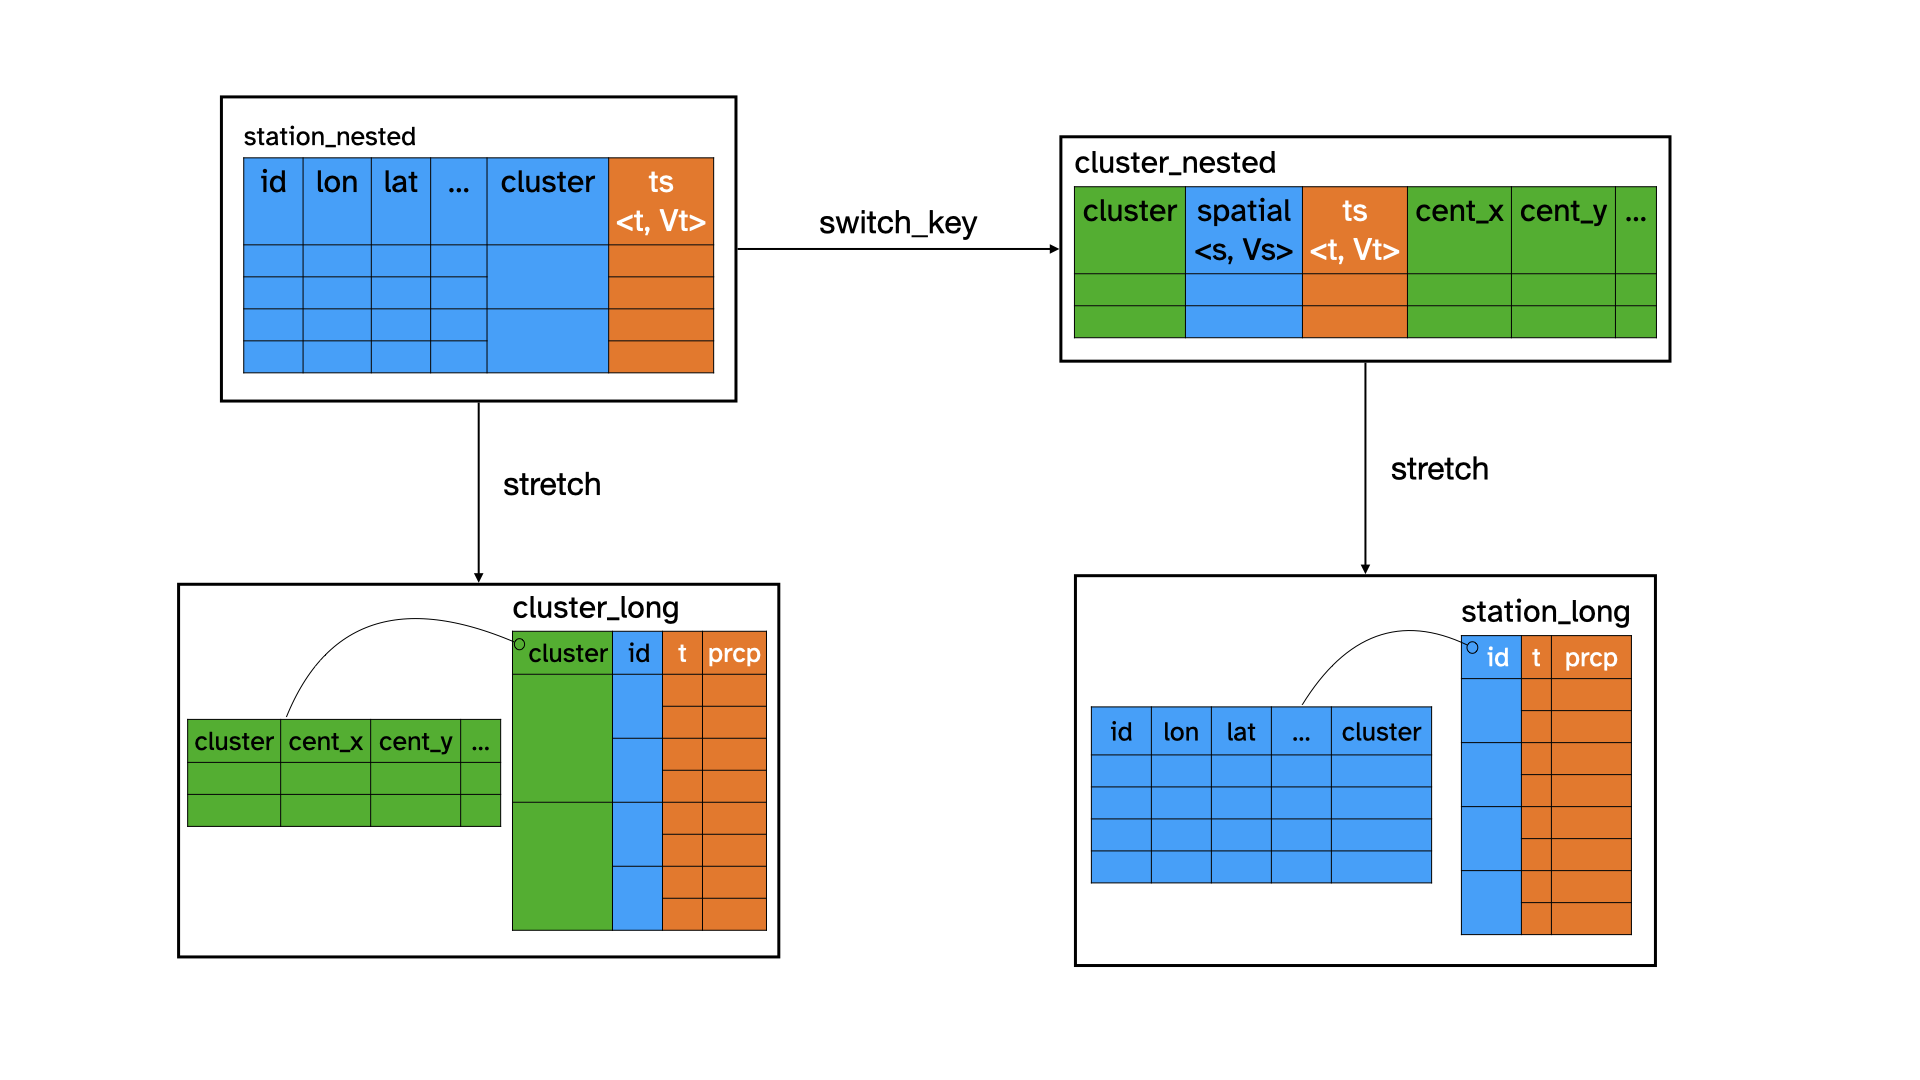
\includegraphics[width=1\linewidth,height=0.4\textheight]{/Users/sherryzhang/Documents/research/paper-cubble/figures/diagram-keynotes/diagram-keynotes.003} 

}

\caption[demon interactivity]{demon interactivity}\label{fig:interactive-workflow}
\end{figure}
\end{CodeChunk}

\newpage

\hypertarget{examples}{%
\section{Examples}\label{examples}}

\hypertarget{australia-precipitation-pattern-in-2020}{%
\subsection{Australia precipitation pattern in
2020}\label{australia-precipitation-pattern-in-2020}}

\hypertarget{basic-manipulation}{%
\subsubsection{Basic manipulation}\label{basic-manipulation}}

Bureau of Meteorology (BoM) collects climate variables. This variables
can be openly queried via \texttt{rnoaa}. \texttt{weatherdata} provides
a readily available copy of several
data.\texttt{weatherdata::historical\_tmax} provides historical maximum
temperature recorded for Australian stations with the earliest dating
back to 1859 and this can be used to understand the change of maximum
temperature from a past period to nowadays. Figure
\ref{fig:glyphmap-workflow} shows the steps involved from the initial
data to the final glyph map in Figure \ref{fig:glyphmap}.

\begin{CodeChunk}
\begin{figure}

{\centering 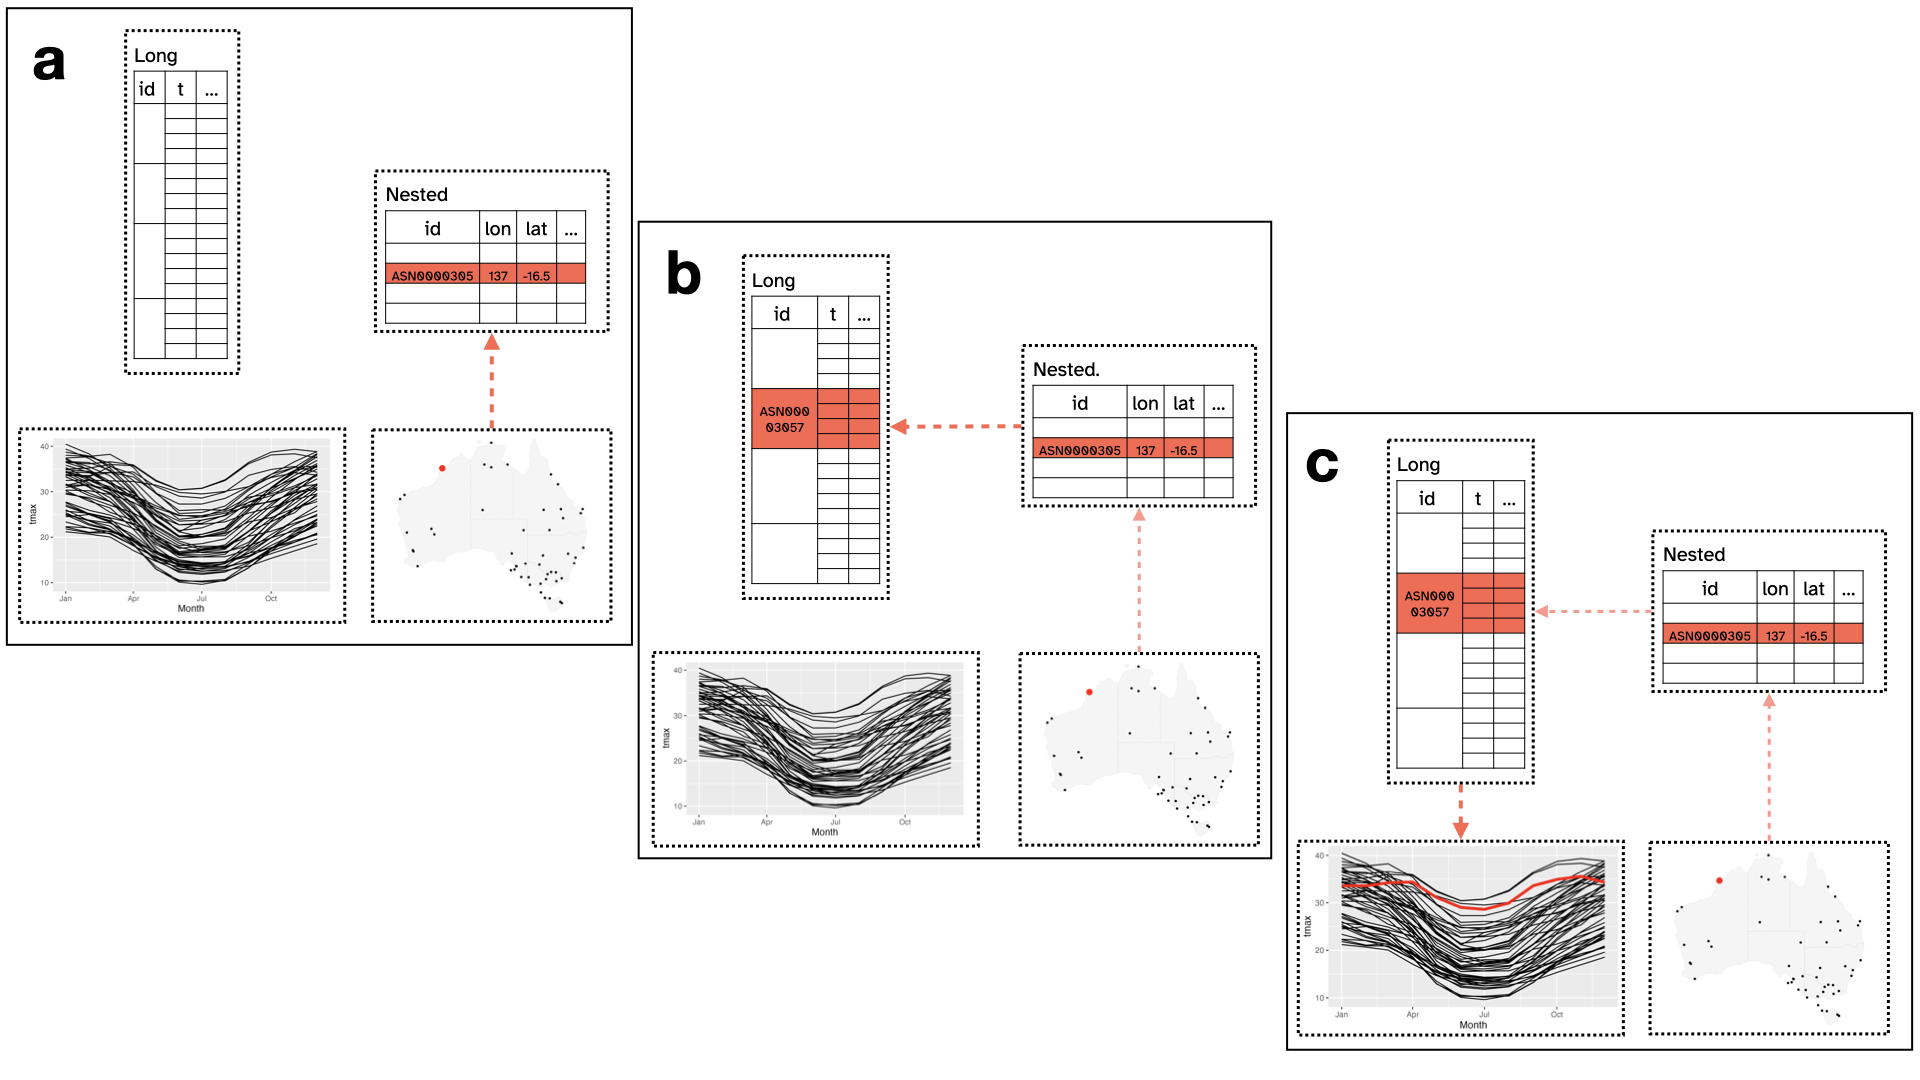
\includegraphics[width=1\linewidth,height=0.4\textheight]{/Users/sherryzhang/Documents/research/paper-cubble/figures/diagram-keynotes/diagram-keynotes.004} 

}

\caption[demon code]{demon code}\label{fig:glyphmap-workflow}
\end{figure}
\end{CodeChunk}

\begin{CodeChunk}
\begin{figure}

{\centering 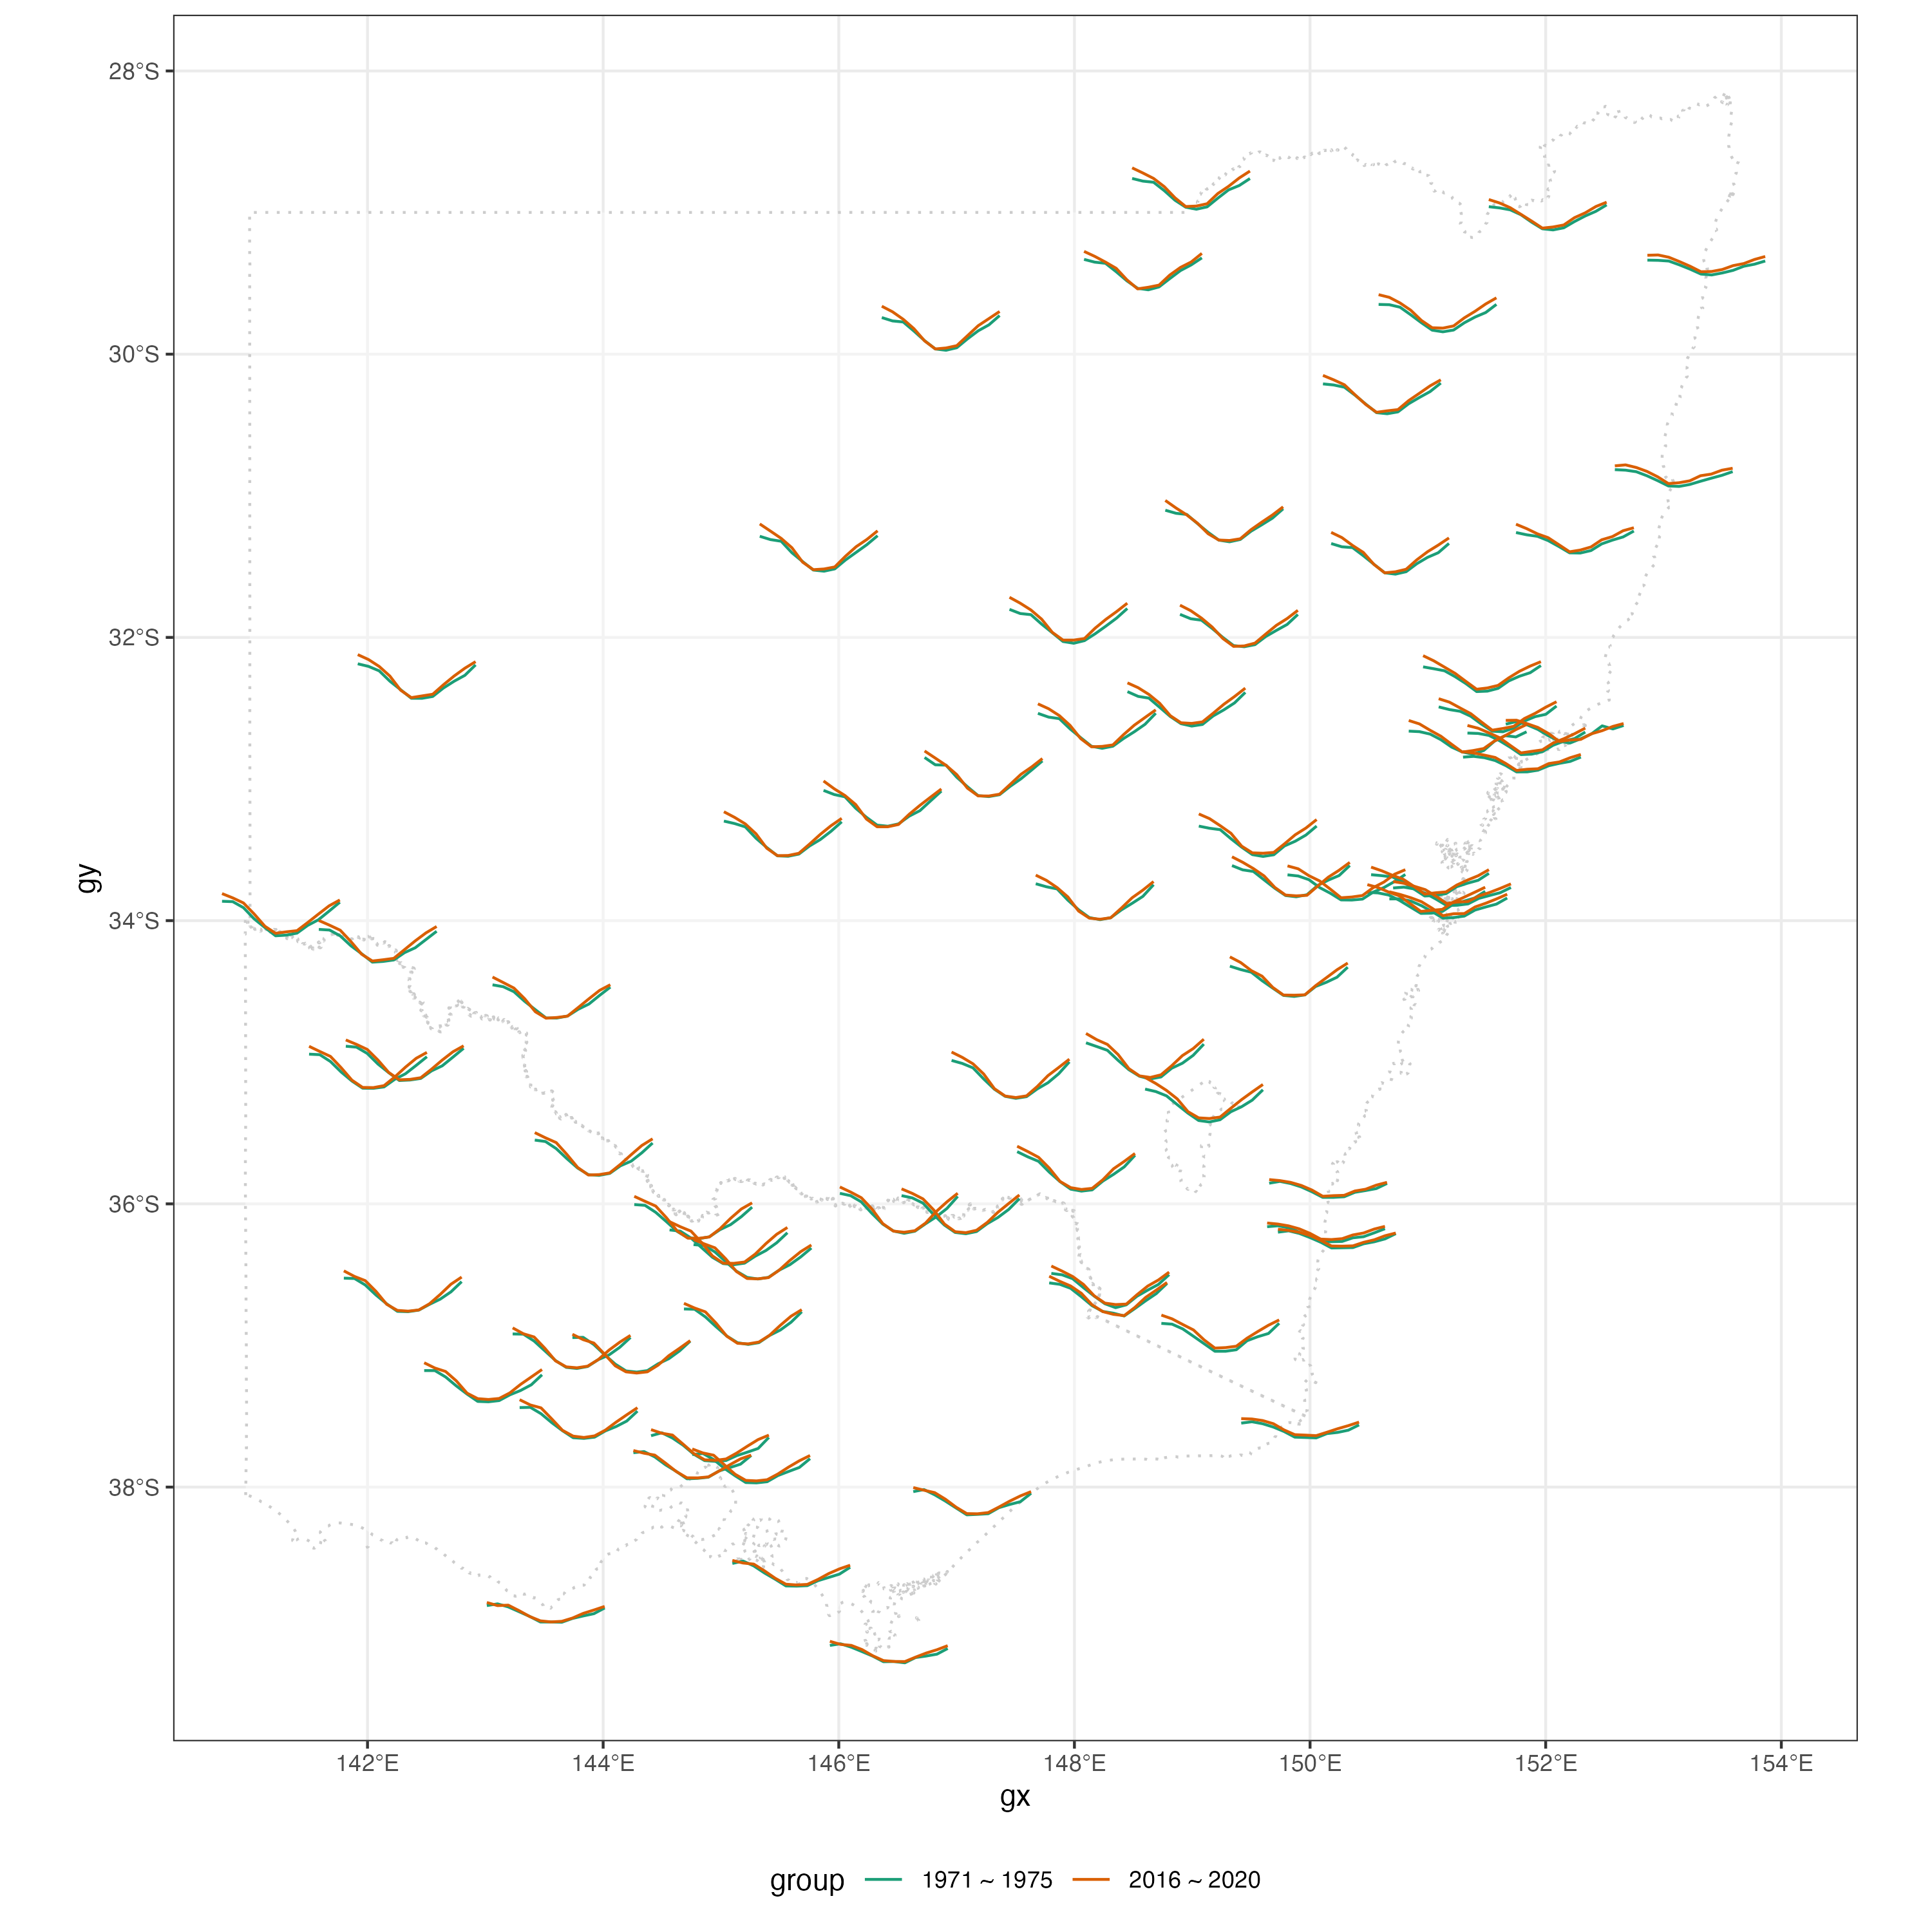
\includegraphics[width=1\linewidth,height=0.7\textheight]{figures/basic-manipulation} 

}

\caption[asdfasd]{asdfasd}\label{fig:glyphmap}
\end{figure}
\end{CodeChunk}

\hypertarget{aggregation}{%
\subsubsection{Aggregation}\label{aggregation}}

In figure \ref{fig:glyphmap}, there are a few stations around Sydney
(151E, 34S) and New castle (152E, 33S). Aggregating them into averages
or other statistics would give a better picture. This can be done with
cubble through a hierarchical structure, where the cluster indicator is
one level above the individual station.

In Figure \ref{fig:aggregation}

The \texttt{weatherdata::climate\_full} data has daily climate data of
639 Australia stations from 2016 to 2020.

calcluate distance matrix As an example to illustrate here, a kmean
clustering algorithm based on the distance matrix is used and the number
of centres is set to 20. More complex algorithms can also be used for
more complex problem, as long as a mapping from each station id to the
cluster id can be constructed.

\begin{CodeChunk}
\begin{figure}

{\centering 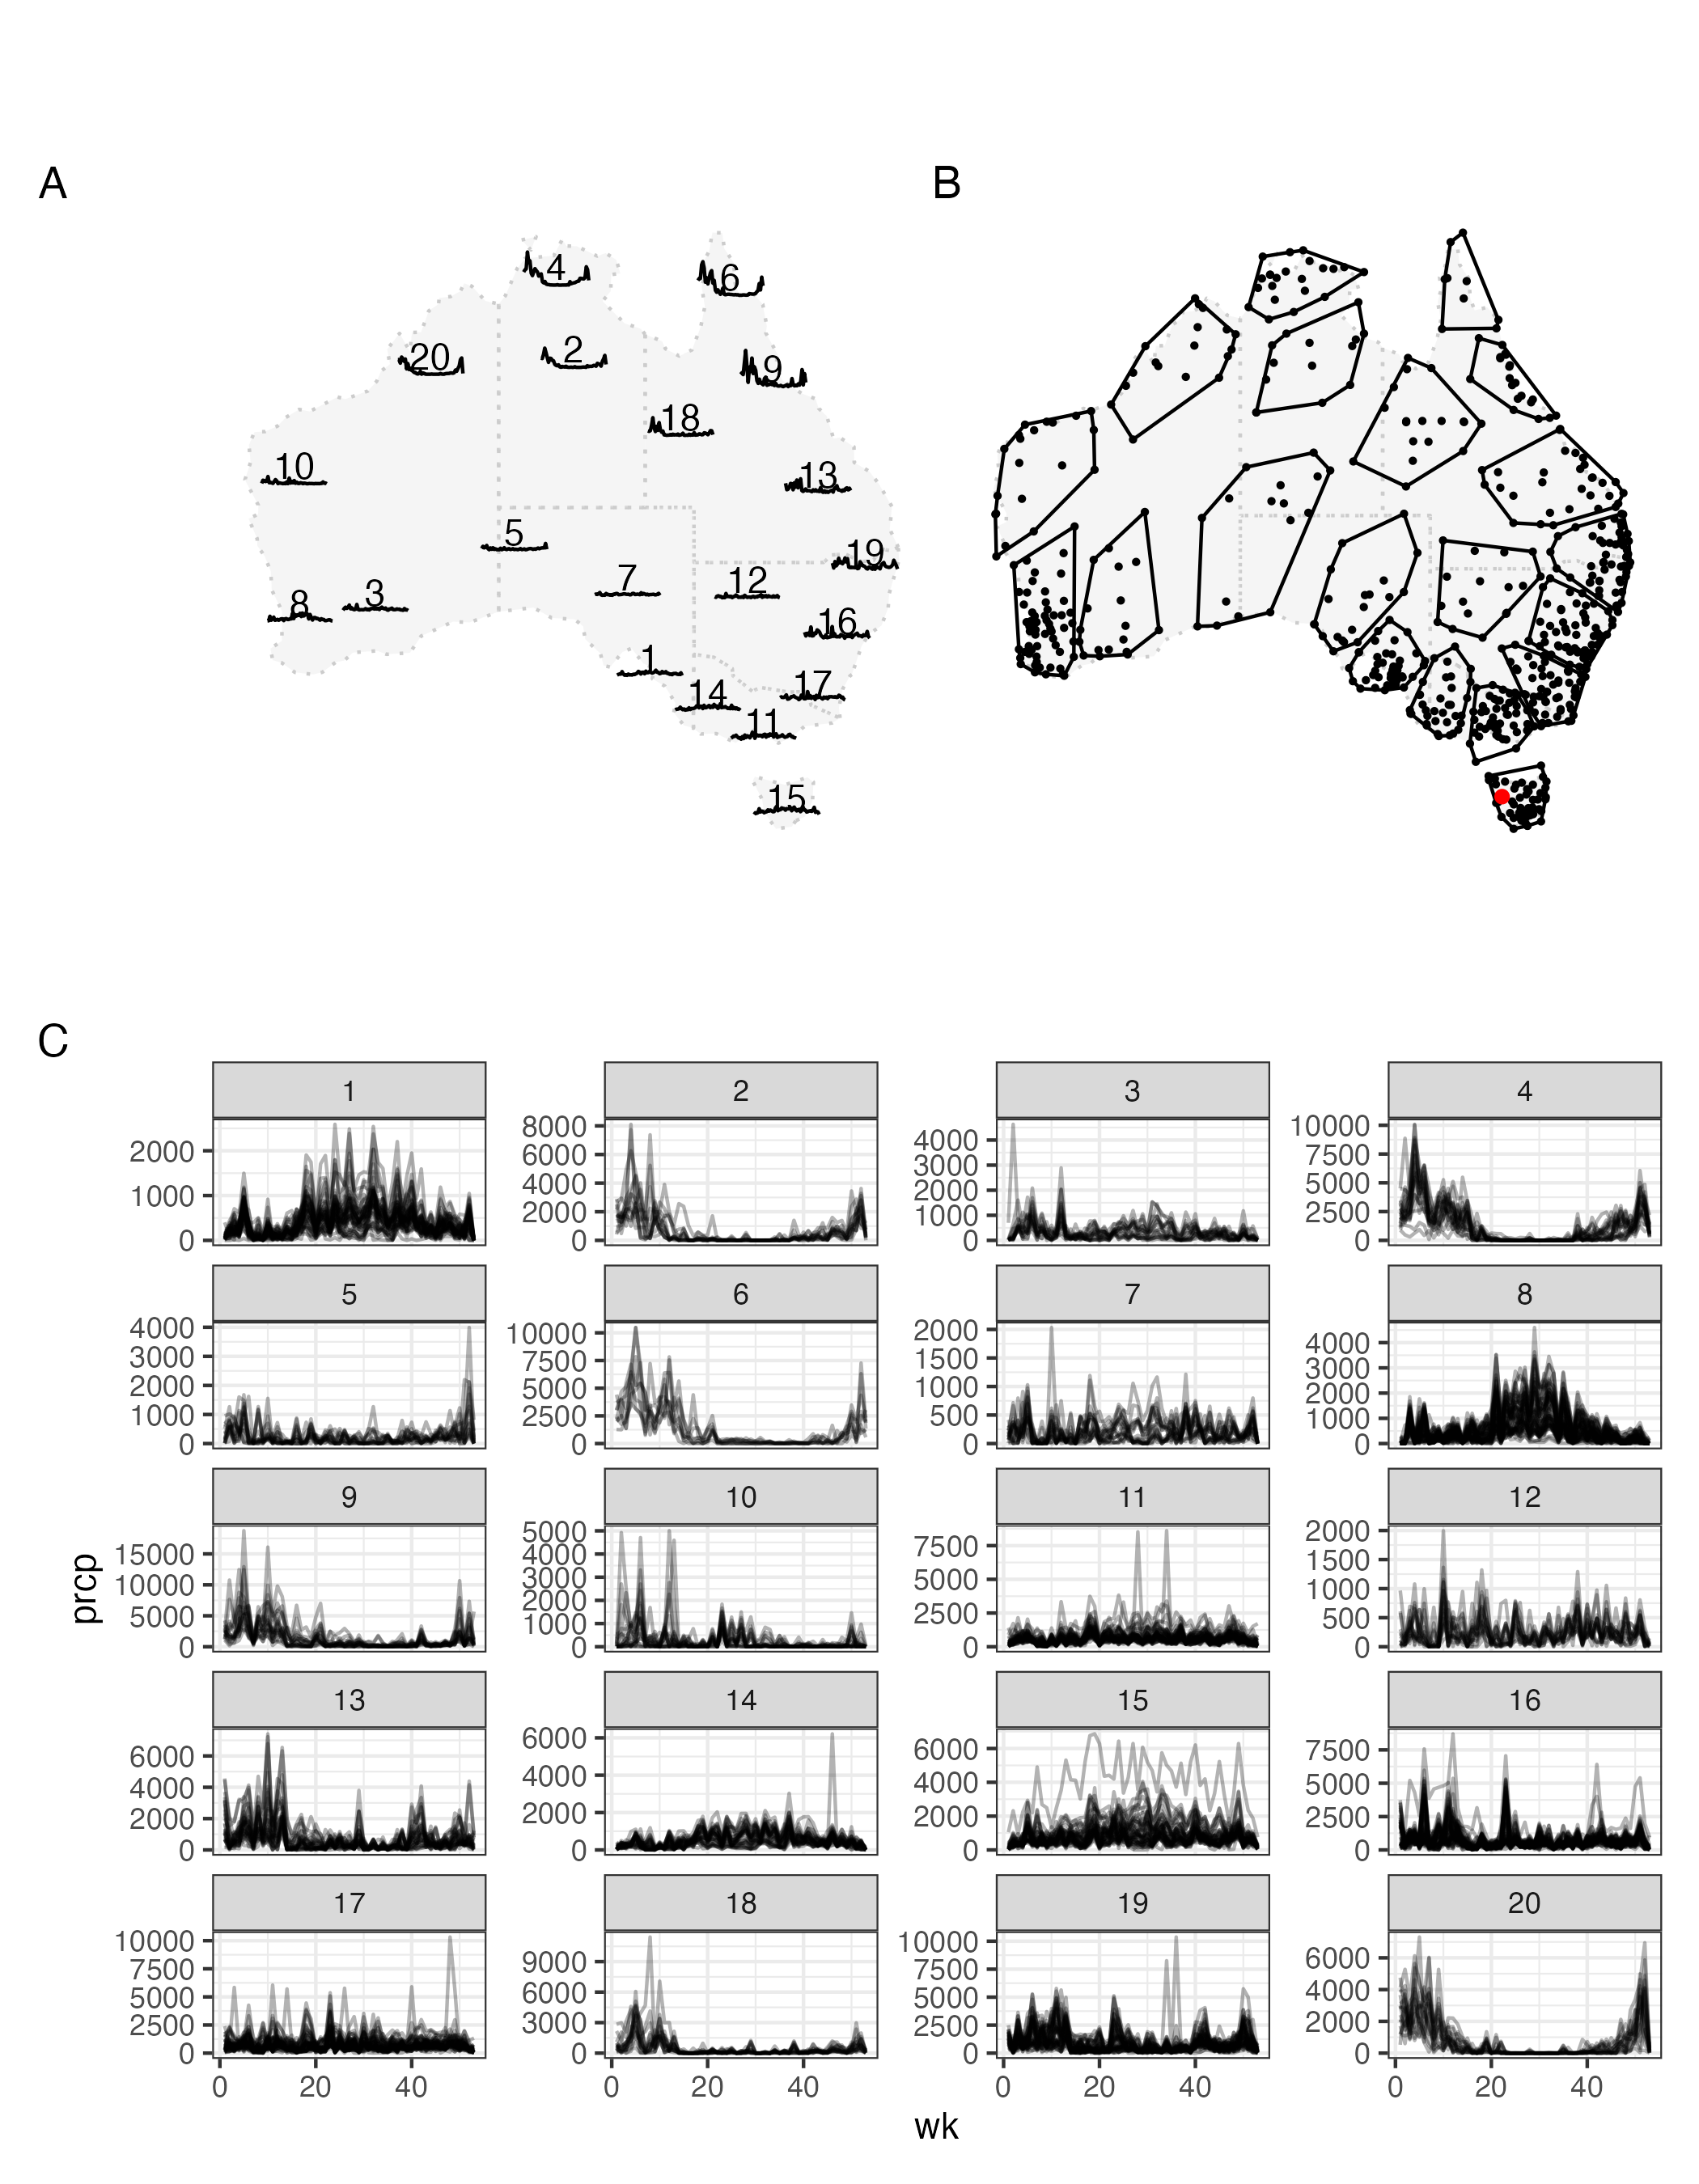
\includegraphics[width=1\linewidth,height=0.9\textheight]{figures/aggregation} 

}

\caption[sdfasdf]{sdfasdf}\label{fig:aggregation}
\end{figure}
\end{CodeChunk}

\hypertarget{river-level-data-in-victria-water-gauges}{%
\subsection{River level data in Victria water
gauges}\label{river-level-data-in-victria-water-gauges}}

The water level data comes from
\href{http://www.bom.gov.au/metadata/catalogue/19115/ANZCW0503900528?template=full}{Bureau
of Meteorology} and has a copy in \texttt{weatherdata}. Here we extract
the water course level and add a column annotate this data of type
\texttt{river}. For the rainfall data, we will still use the
\texttt{weatherdata::climate\_full}, filtering for Victorian stations in
2020 should be pretty familiar by now. Again, we first look at where
these stations are on the map first:

\begin{CodeChunk}


\begin{center}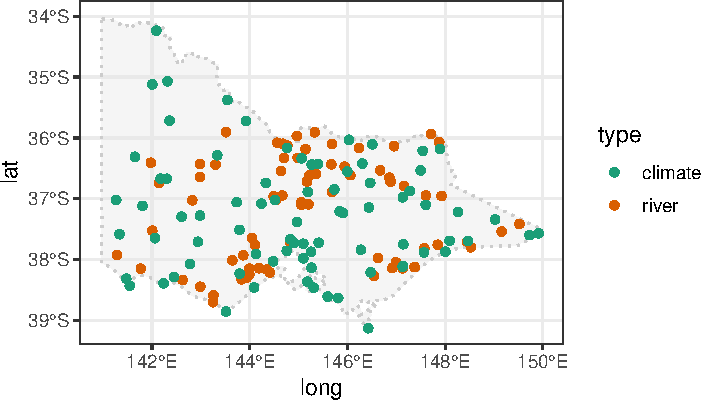
\includegraphics{figures/unnamed-chunk-7-1} \end{center}

\end{CodeChunk}

Temporal matching checks how spatially matched pairs align temporally.
We use the following chart to illustrate how the temporal matching
works:

\begin{CodeChunk}
\begin{figure}

{\centering 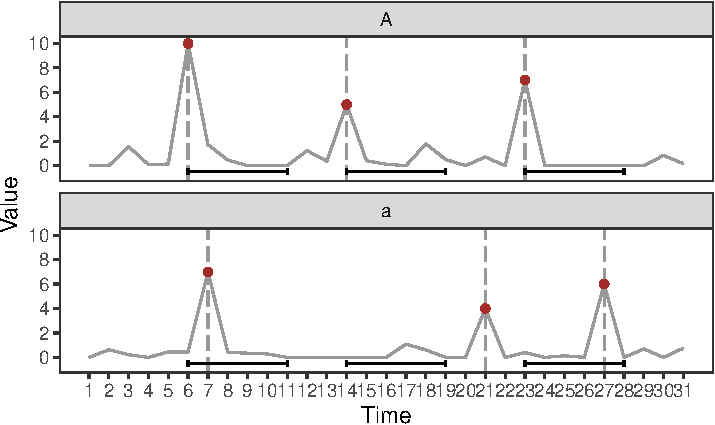
\includegraphics{figures/unnamed-chunk-8-1} 

}

\caption[shtishisaasdf]{shtishisaasdf}\label{fig:unnamed-chunk-8}
\end{figure}
\end{CodeChunk}

For each spatially matched pair, say \texttt{A} and \texttt{a}, we first
find the largest \texttt{n} points in each series, colored in brown
points here. Here we use the largest three but you can tune this number
by \texttt{temporal\_n\_highest}. Then we construct the interval of the
largest points from one series and see how many points, from the other
series, fall into the intervals. The series used to construct the
interval is controlled by \texttt{temporal\_independent} and the window
size by \texttt{temporal\_window} with a default of 5.

In this illustration, we construct the interval based on series
\texttt{A} and two of the three peaks from \texttt{a} falls into this
interval at Time 7 and 27.

There's another mandatory argument that hasn't been introduced above:
\texttt{temporal\_var\_to\_match}. This argument controls the variable
to match and it needs to appear in both the \texttt{major} and
\texttt{minor} set. In the water level matching example, we match the
variable \texttt{Water\_course\_level} from \texttt{river} to
\texttt{prcp} from \texttt{climate}, hence need to manually rename one
of them to match the other, here we rename \texttt{Water\_course\_level}
to \texttt{prcp} in \texttt{river}:

Now we use \texttt{match\_sites()} to first pair the weather stations
with the river gauges spatially and then apply the temporal matching on
\texttt{prcp}. We will construct the interval based on peaks in
\texttt{climate} since we would expect a lag effect for precipitation to
flow into the river and cause a raise in river level, hence
\texttt{temporal\_independent\ =\ climate}. We select the 30 highest
peak from the series to construct the match by setting
\texttt{temporal\_n\_highest\ =\ 30}. This is a tuning parameter and you
can start with 10\% of the points of one series (here we have daily data
for a year, 10\% is roughly 30 points). \texttt{temporal\_min\_match}
filters out pairs don't have enough match and to return all the pairs,
set \texttt{temporal\_min\_match} to \texttt{0}.

\begin{CodeChunk}
\begin{CodeOutput}
# cubble:   id [8]: nested form
# bbox:     [144.52, -37.73, 146.06, -36.55]
# temporal: date [date], prcp [dbl]
  id          name                lat  long type  ts        .dist .group n_match
  <chr>       <chr>             <dbl> <dbl> <chr> <list>    <dbl>  <int>   <int>
1 405234      SEVEN CREEKS @ D~ -36.9  146. river <tibble ~  6.15      5      21
2 ASN00082042 strathbogie       -36.8  146. clim~ <tibble ~  6.15      5      21
3 404207      HOLLAND CREEK @ ~ -36.6  146. river <tibble ~  8.54     10      21
4 ASN00082170 benalla airport   -36.6  146. clim~ <tibble ~  8.54     10      21
5 230200      MARIBYRNONG RIVE~ -37.7  145. river <tibble ~  6.17      6      19
6 ASN00086038 essendon airport  -37.7  145. clim~ <tibble ~  6.17      6      19
7 406213      CAMPASPE RIVER @~ -37.0  145. river <tibble ~  1.84      1      18
8 ASN00088051 redesdale         -37.0  145. clim~ <tibble ~  1.84      1      18
\end{CodeOutput}
\end{CodeChunk}

The output from temporal matching is also a cubble, with additional
column \texttt{.dist} and \texttt{.group} inherent from spatial matching
and \texttt{n\_match} for the number of matched temporal peaks. Then you
can use this output to plot the location of match or to look at the
series:

\begin{CodeChunk}
\begin{figure}

{\centering 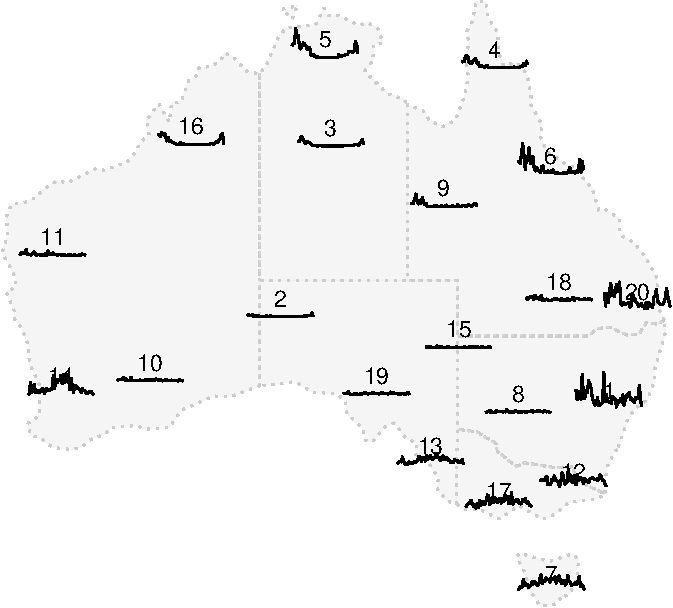
\includegraphics[width=1\linewidth]{figures/unnamed-chunk-11-1} 

}

\caption[..]{...}\label{fig:unnamed-chunk-11}
\end{figure}
\end{CodeChunk}

\hypertarget{era5-climate-reanalysis-data}{%
\subsection{ERA5: climate reanalysis
data}\label{era5-climate-reanalysis-data}}

\hypertarget{interative-graphic-with-cubble}{%
\subsection{Interative graphic with
cubble}\label{interative-graphic-with-cubble}}

\begin{CodeChunk}


\begin{center}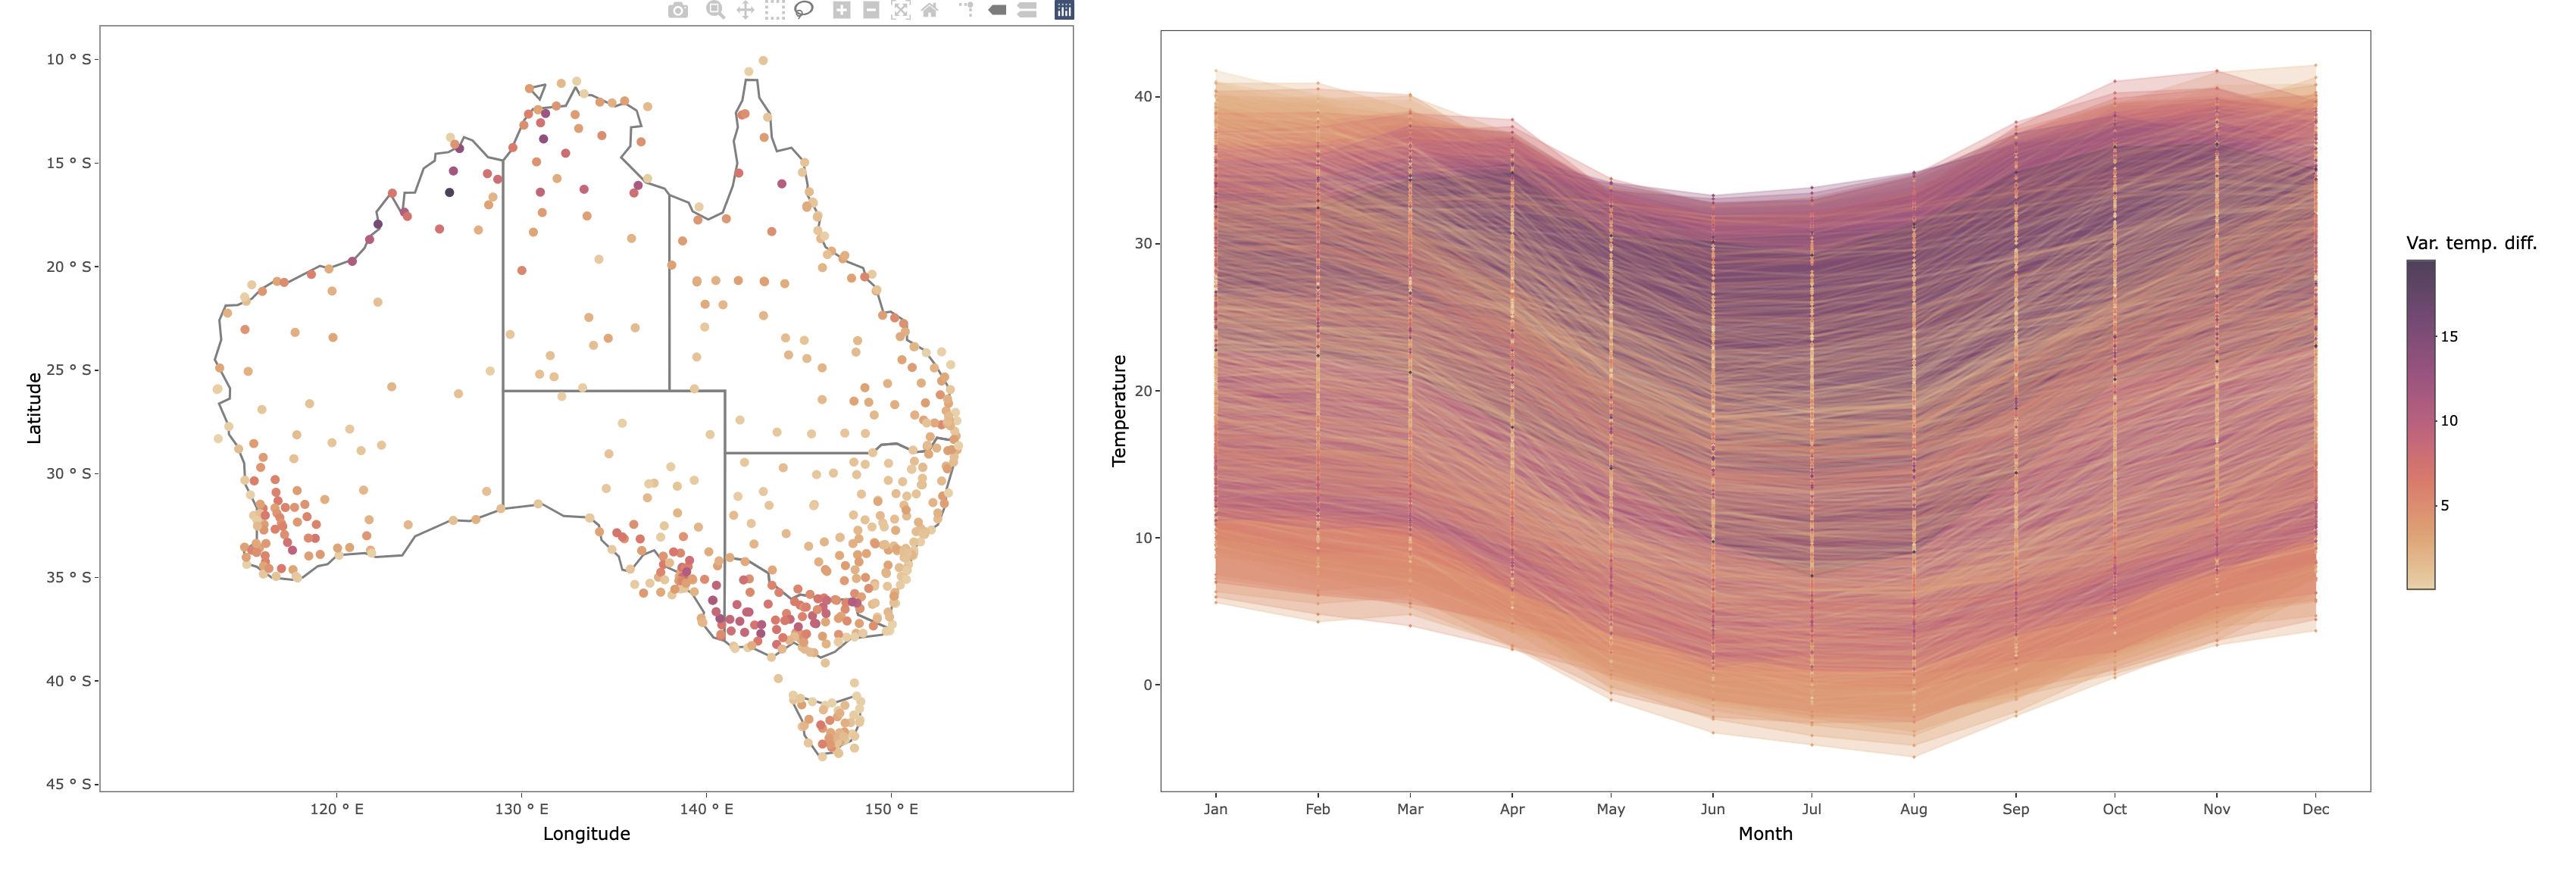
\includegraphics[width=1\linewidth,height=0.3\textheight]{/Users/sherryzhang/Documents/research/paper-cubble/figures/linking} \end{center}

\end{CodeChunk}

\begin{CodeChunk}


\begin{center}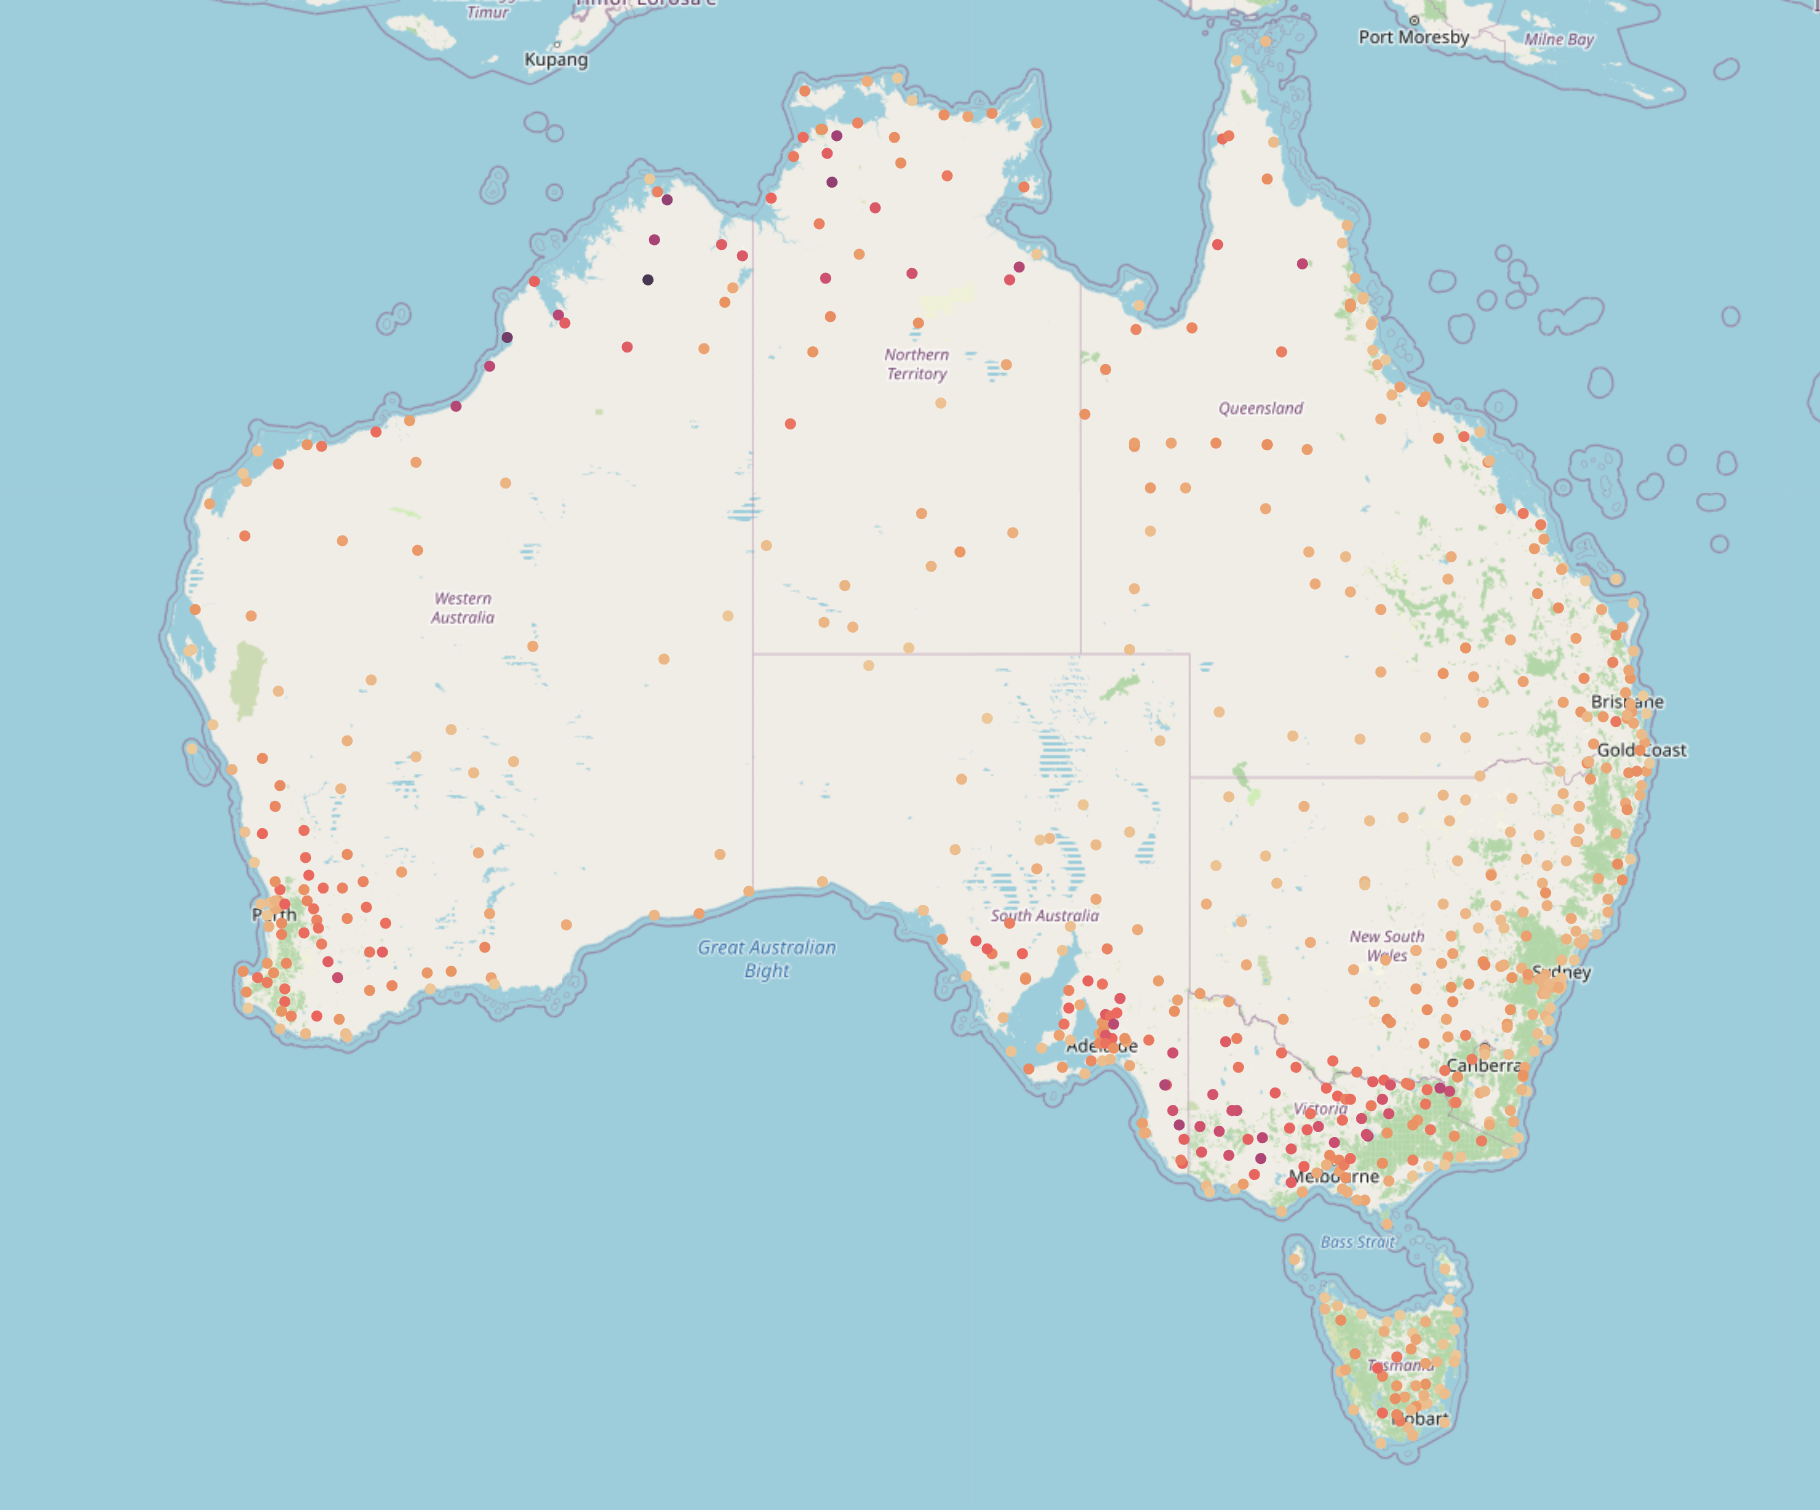
\includegraphics[width=0.5\linewidth,height=0.3\textheight]{/Users/sherryzhang/Documents/research/paper-cubble/figures/popup} \end{center}

\end{CodeChunk}

\hypertarget{conclusion}{%
\section{Conclusion}\label{conclusion}}

\newpage

\hypertarget{old-stuff}{%
\section{Old stuff}\label{old-stuff}}

In the temporal aspect, the \texttt{tsibble} \citep{tsibbles} structure
and its tidyverts ecosystem have provided a {[}\ldots{} {]} workflow to
work with temporal data. In a tsibble structure, temporal data is
characterised by \texttt{index} and \texttt{key} where \texttt{index} is
the temporal identifier and \texttt{key} is the identifier for multiple
series, which could be used as a spatio identifier. However, a tsibble
object, by construction, always requires the \texttt{index} in its
structure. This makes it less appealing for spatio-temporal data since
the output of calculated spatio-specific variables (i.e.~features of
each series) don't have the time dimension. Analysts will either need to
have an additional step to join this output to the original tsibble or
operate with variables stored in two separate objects. In addition, the
long form structure of a tsibble object means spatio variables
(i.e.~longitude, latitude, and features of each series if joined back to
the tsibble) of each spatio identifier will be repetitively recorded at
each timestamp. This repetition is unnecessary and would inflate the
object size for long series.

\hypertarget{create-a-cubble}{%
\section{Create a cubble}\label{create-a-cubble}}

The creation of a cubble requires the site identifier (\texttt{key}), as
well as the spatial (\texttt{coords}) and temporal (\texttt{index})
identifier. \texttt{climate\_flat} is already a tibble and it uses
\texttt{id} to identify each station, \texttt{date} as the time
identifier, and \texttt{c(long,\ lat)} as the spatial identifier. To
create a cubble for this data, use:

\begin{CodeChunk}
\begin{CodeOutput}
# cubble:   id [5]: nested form
# bbox:     [115.97, -32.94, 133.55, -12.42]- check gap on long and lat
# temporal: date [date], prcp [dbl], tmax [dbl], tmin [dbl]
  id            lat  long  elev name           wmo_id ts                
  <chr>       <dbl> <dbl> <dbl> <chr>           <dbl> <list>            
1 ASN00009021 -31.9  116.  15.4 perth airport   94610 <tibble [366 x 4]>
2 ASN00010311 -31.9  117. 179   york            94623 <tibble [366 x 4]>
3 ASN00010614 -32.9  117. 338   narrogin        94627 <tibble [366 x 4]>
4 ASN00014015 -12.4  131.  30.4 darwin airport  94120 <tibble [366 x 4]>
5 ASN00015131 -17.6  134. 220   elliott         94236 <tibble [366 x 4]>
\end{CodeOutput}
\end{CodeChunk}

Most of the time, spatio-temporal data doesn't come into this form and
analysts need to query the climate variables based on station metadata.
\textcolor{red}{This is also a problem illustrated in Section 3.5 in @tidydata. Here we provide a structured way to query this data based on the row-wise operator and nested list.}
For this type of task, one can structure a metadata into a tibble and
use row-wise operator to query the climate variables into a nested list.
As an example here we demonstrate the workflow to find the 5 closest
stations to Melbourne. We first create a station data frame with the 5
target stations.

\begin{CodeChunk}
\begin{CodeOutput}
# A tibble: 5 x 8
  id            lat  long  elev name                 wmo_id  dist city     
  <chr>       <dbl> <dbl> <dbl> <chr>                 <dbl> <dbl> <chr>    
1 ASN00086038 -37.7  145.  78.4 essendon airport      95866  10.8 melbourne
2 ASN00086282 -37.7  145. 113.  melbourne airport     94866  20.1 melbourne
3 ASN00086077 -38.0  145.  12.1 moorabbin airport     94870  21.9 melbourne
4 ASN00088162 -37.4  145. 528.  wallan (kilmore gap)  94860  48.1 melbourne
5 ASN00087113 -38.0  144.  10.6 avalon airport        94854  48.8 melbourne
\end{CodeOutput}
\end{CodeChunk}

We can query the climate information into a nested list named
\texttt{ts} for each station with the \texttt{rowwise()} operator. To
create a cubble, supply the same identifiers as with the first example.

\begin{CodeChunk}
\begin{CodeOutput}
# cubble:   id [5]: nested form
# bbox:     [144.47, -38.03, 145.1, -37.38]
# temporal: date [date], prcp [dbl], tmax [dbl], tmin [dbl]
  id            lat  long  elev name                 wmo_id  dist city   ts     
  <chr>       <dbl> <dbl> <dbl> <chr>                 <dbl> <dbl> <chr>  <list> 
1 ASN00086038 -37.7  145.  78.4 essendon airport      95866  10.8 melbo~ <tibbl~
2 ASN00086282 -37.7  145. 113.  melbourne airport     94866  20.1 melbo~ <tibbl~
3 ASN00086077 -38.0  145.  12.1 moorabbin airport     94870  21.9 melbo~ <tibbl~
4 ASN00088162 -37.4  145. 528.  wallan (kilmore gap)  94860  48.1 melbo~ <tibbl~
5 ASN00087113 -38.0  144.  10.6 avalon airport        94854  48.8 melbo~ <tibbl~
\end{CodeOutput}
\end{CodeChunk}

Below are the how the nested and long form look like for Australia
climate data, which records daily precipitation, maximum and minimum
temperature for 55 stations across Australia from 2015- 2020. Notice
that each station forms a group in both forms and specifically, the
nested and long form have a underlying \texttt{rowwise\_df} and
\texttt{grouped\_df} respectively.

With a cubic framework on mind, different types of manipulation with
cubble can be thought of as slicing the cube in various way. The table
below shows how some \texttt{dplyr} verbs are mapped into the operation
in a cubble. With the existing grouping on the station, additional
grouping can be added with \texttt{group\_by} and removed with
\texttt{ungrouped}. {[}talk about why it is useful{]}

\newpage

\hypertarget{cubble-operations}{%
\subsection{Cubble operations}\label{cubble-operations}}

\begin{CodeChunk}
\begin{figure}

{\centering 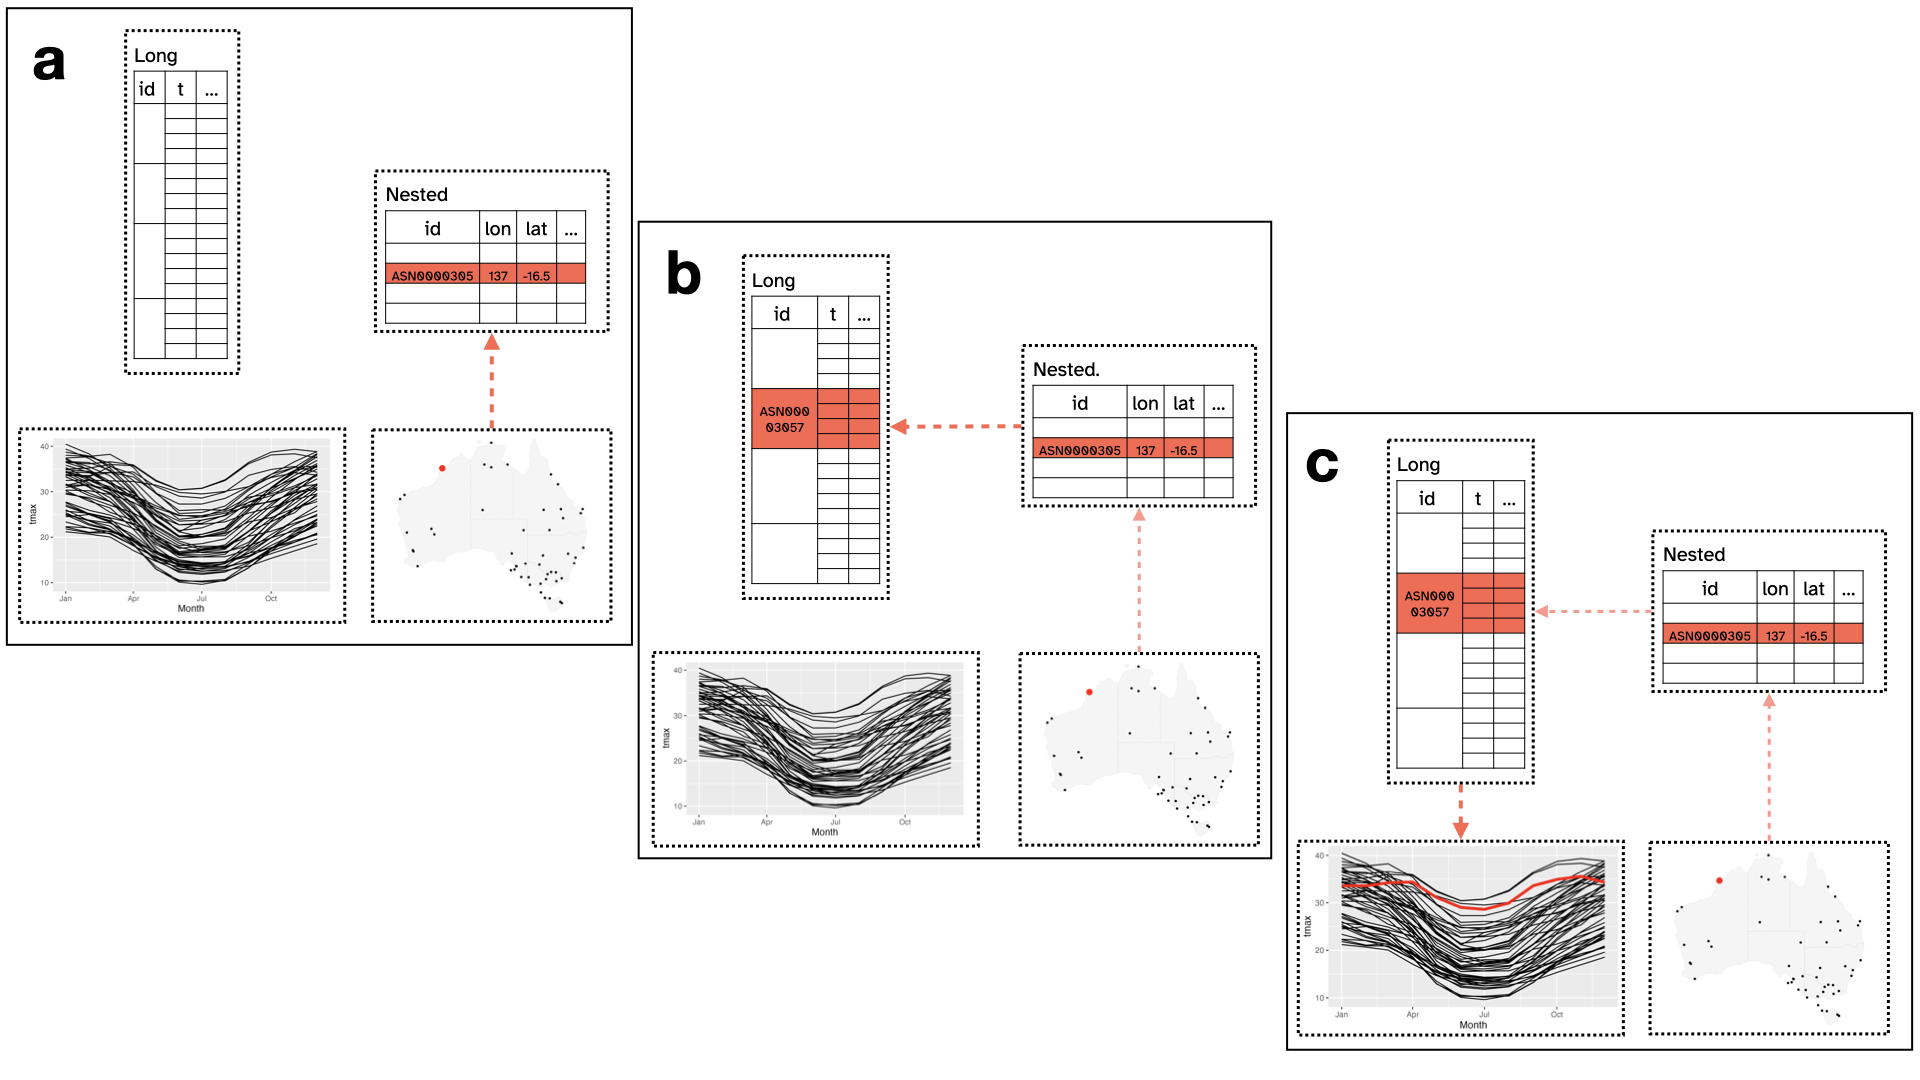
\includegraphics[width=0.9\linewidth,height=0.5\textheight]{/Users/sherryzhang/Documents/research/paper-cubble/figures/diagram-keynotes/diagram-keynotes.004} 

}

\caption[Cubble operations]{Cubble operations}\label{fig:cubble-operations}
\end{figure}
\end{CodeChunk}

\bibliography{references.bib}


\end{document}
